\section{Pianificazione e interazioni con il \textit{tutor}}
All'inizio dello \stage{} ho avuto un incontro con il \textit{tutor} aziendale, per discutere del piano di lavoro, e per definire la modalità
di svoldimento e di interazione durante lo \stage.\\
Abbiamo deciso di fare un incontro settimanale, per discutere delle attività svolte durante la settimana, e per pianificare le attività
della settimana successiva.\\
Quando avevo dei dubbi o dei problemi, potevo contattarelo tramite Google Chat o tramite \textit{email}.\\
Ogni mattina alle 9:00 avevamo un incontro con il \textit{team} di sviluppo, per discutere delle attività svolte il giorno precedente, e per
pianificare le attività della giornata, come previsto dalla metodologia \textit{Agile} e illustrato in figura \ref*{fig:scrum_agile}).\\
A questo incontro non partecipava il \textit{tutor} aziendale. 
Capitava spesso comunque di avere degli incontri al di fuori di quelli pianificati, per discutere di problemi, principalmente analitici, 
e per prendere decisioni riguardanti l'implementazione.\\

\begin{figure}[h] 
  \centering 
  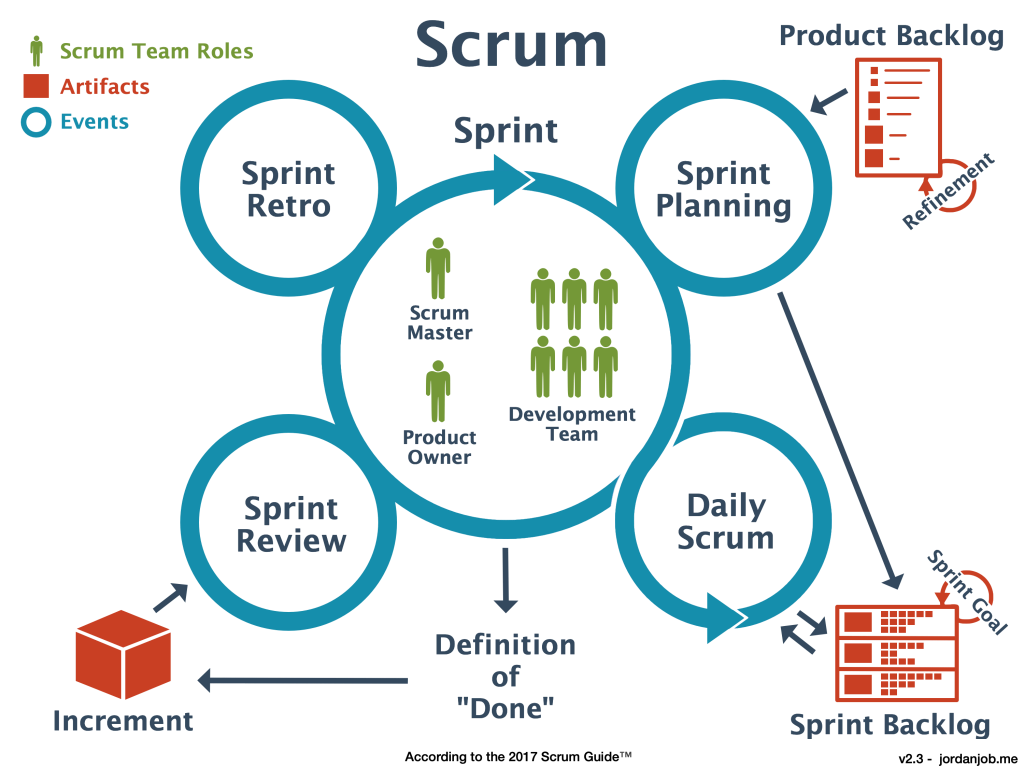
\includegraphics[width=.8\columnwidth]{scrum_agile.png} 
  \caption{Metodologia \textit{Agile}. Fonte: https://jordanjob.me/blog/scrum-diagram. }
  \label{fig:scrum_agile}
\end{figure}